\documentclass[11pt,twoside]{scrartcl}
%\documentclass[11pt,twoside]{article}

%opening
\newcommand{\lecid}{15-316}
\newcommand{\leccourse}{Software Foundations of Security and Privacy}
\newcommand{\lecdate}{} %e.g. {October 21, 2013}
\newcommand{\lecnum}{18}
\newcommand{\lectitle}{Provable Privacy}
\newcommand{\lecturer}{Matt Fredrikson}
\newcommand{\lecurl}{https://15316-cmu.github.io/index}

\usepackage{varwidth}
\usepackage{lecnotes}
\usepackage[irlabel]{bugcatch}

\usepackage{tikz}
\usetikzlibrary{automata,shapes,positioning,matrix,shapes.callouts,decorations.text,patterns,decorations.pathreplacing}
\usepackage{pgfplots}

% \usepackage[bracketinterpret,seqinfers,sidenotecalculus]{logic}
% \newcommand{\I}{\interpretation[const=I]}

% \newcommand{\bebecomes}{\mathrel{::=}}
% \newcommand{\alternative}{~|~}
% \newcommand{\asfml}{F}
% \newcommand{\bsfml}{G}
% \newcommand{\cusfml}{C}
% \def\sqsubseteqftrule{L}%
% \def\rightrule{R}%

\pgfplotsset{compat=1.10}
\pgfmathdeclarefunction{gauss}{2}{%
  \pgfmathparse{1/(#2*sqrt(2*pi))*exp(-((x-#1)^2)/(2*#2^2))}%
}

\pgfmathdeclarefunction{laplace}{1}{%
  \pgfmathparse{1/(2*#1)*exp(-abs(x)/#1)}%
}

\pgfmathdeclarefunction{biaslaplace}{2}{%
  \pgfmathparse{1/(2*#2)*exp(-abs(x - #1)/#2)}%
}

\begin{document}

\newcommand{\atrace}{\omega}%
%% the standard interpretation naming conventions
\newcommand{\stdI}{\dTLint[state=\omega]}%
\newcommand{\Ip}{\dTLint[trace=\atrace]}%
\newcommand{\ws}{\omega}\newcommand{\wt}{\nu}% 

\maketitle
\thispagestyle{empty}

%%%%%%%%%%%%%%%%%%%%%%%%%%%%%%%%%%%%%%%%%%%%%%

\section{Introduction}

In today's lecture, we will look more carefully at a different set of techniques for revealing some useful information about secret state while controlling the attacker's level of uncertainty about it. These techniques all use randomness to produce approximate results for computations, while providing some form of cover for the true secret. We will look at a property called \emph{differential privacy}~\cite{dwork06} that formalizes the protections one might gain from this approach, and study some properties that make it useful for building computations that protect secret data. Differential privacy has been applied to a wide range of important computations to protect the privacy of source data~\cite{Dwork2014}, from machine learning~\cite{Chaudhuri2011} to web browser data collection~\cite{ErlingssonKP14}. We will not have time to cover these applications in any detail, but will instead focus on the core ideas behind the approach.

\section{Quantifying uncertainty}

% In the previous lecture we mentioned that when the feasible set is large, it is an indication that the associated program did not reveal ``too much'' about its secret initial state. The reason for this is that when a large number of initial states remain consistent with an attacker's observations, then the attacker's uncertainty about which one was actually used is great. So perhaps we can reason about information flow security in terms of keeping the attacker's uncertainty about the secret high.

% One way of quantifying uncertainty regarding which of a set of events occurred is to assign numeric values to each event that correspond to one's assessment of their probability. In this case we would like to characterize the attacker's uncertainty, and the set of ``events'' that the attacker is uncertain about is which initial state $\asprg$ was executed on. We will use standard probability measures to quantify the attacker's level of uncertainty about particular candidates for the initial state. So for example, if the attacker is absolutely certain that the initial state was $\omega_i$, then they would assign the probability $\pr[\omega_i] = 1$, and $\pr[\omega_j] = 0$ for all $j \ne i$. Or supposing that there are $N$ possible states and the attacker deems them all equally likely (i.e., their uncertainty is very great), then $\pr[\omega_i] = 1/N$ for all $i$.

What can we do if the program that we want to write is inherently ``leaky''? One way that we can make the attacker more uncertain about the secret initial state is to use randomness in our program. Consider for example a technique called \emph{randomized response}~\cite{Warner1965}, which is a privacy technique dating back to the 1960s with roots in the social sciences. Randomized response was motivated by survey collection, in situations where questions asked of respondents relate to sensitive issues. Randomized response gives these subjects \emph{plausible deniability}, by providing a structured way of adding random ``noise'' to their answer.

In the following, assume that $\flip(p)$ is a random function that flips a biased coin with parameter $p$. In other words,
\begin{equation}
\flip() = 
\left\{
\begin{array}{ll}
%
1 & \mathrm{with\ probability\ } 1/2 \\
0 & \mathrm{with\ probability\ } 1/2
\end{array}
\right.
\end{equation}
Then suppose that $F$ is a function that returns a value in $\{0,1\}$, and that we wish to release $F(x)$ publicly while hiding the secret value $x$ as much as possible. Then the randomized response program $\mathsf{RandResp}$, is as follows, where we assume that the variable $o$ is publicly-observable and $b$ is not (e.g., $\Gamma = x : \hisec, b : \hisec, o : \lowsec)$.
\begin{equation}
\begin{array}{l}
%
b := \flip() \\
\mathbf{if}\ b = 1\ \mathbf{then} \\
\ \ o := F(x) \\
\mathbf{else} \\
\ \ o := \flip()
\end{array}
\end{equation}
In short, randomized response returns the true value of $F(x)$ with probability 1/2, and a completely random answer with probability 1/2. In terms of feasible sets, this appears to be an absolutely brilliant approach because now the attacker must be completely uncertain about the initial value of $x$. Why is this so? The adversary can only see $o$, and if $b = 0$ after being assigned, then $o$ does not depend at all on $x$, so $x$ could be anything as though the program satisfied non-interference.

But perhaps this doesn't seem quite right. Let's assume for a moment that $x \in \{0,1\}$ and $F$ is simply the identity function, and walk through the various possibilities. In the following, we will treat $\mathsf{RandResp}$ as though it were a function of $x$ that returns the value in $o$ after executing. If $x = 0$, then,
\begin{equation}
\pr[\mathsf{RandResp}(0) = 0] = \pr[b = 1] + \pr[b = 0 \land \flip() = 0] = 1/2 + 1/4 = 3/4
\end{equation}
We could use the exact same reasoning to conclude that $\pr[\mathsf{RandResp}(1) = 1] = 3/4$. Likewise we could reason about the probability that randomized response outputs an incorrect answer,
\begin{equation}
\pr[\mathsf{RandResp}(0) = 1] = 1 - \pr[\mathsf{RandResp}(0) = 0] = \pr[b = 0 \land \flip() = 1] = 1/4
\end{equation}
So we see that $\mathsf{RandResp}$ outputs the \emph{correct} value of $F(x)$ with fairly high probability of 3/4, and an incorrect ``random'' value with probability 1/4. In other words, most of the time the attacker is safe in assuming that $\mathsf{RandResp}$ outputs exactly the same value as $F(x)$, and so can go about inferring $x$ by computing feasible sets as before. 

This isn't to say that randomized response does nothing to protect $x$, and indeed it may offer ample protection for many applications because the attacker still has more uncertainty than they would otherwise. But by reasoning about the probabilities of various outcomes and what the attacker is able to infer from them, we arrived at a much more nuanced view of the degree of security than was suggested by looking at the feasible set of $\mathsf{RandResp}$ alone.

\subsection{Quantifying a tradeoff}

There are some arbitrary choices that have been made in this conception of randomized response, and they influence the degree of adversarial uncertainty of the secret input $x$. In particular, we could generalize $\flip()$ by adding a parameter $0 \le p \le 1$ controlling the bias of the coin.
\begin{equation}
\flip(p) = 
\left\{
\begin{array}{ll}
%
1 & \mathrm{with\ probability\ } p \\
0 & \mathrm{with\ probability\ } 1 - p
\end{array}
\right.
\end{equation}
We could use this in $\mathsf{RandResp}$ as follows, assuming $p$ is chosen to be some constant in advance.
\begin{equation}
\begin{array}{l}
%
b := \flip(p) \\
\mathbf{if}\ b = 1\ \mathbf{then} \\
\ \ o := F(x) \\
\mathbf{else} \\
\ \ o := \flip(p)
\end{array}
\end{equation}
Then updating the analysis we did before with this more general solution, we see that:
\begin{multline}
\pr[\mathsf{RandResp}(x) = F(x)] = \pr[b = 1] + \pr[b = 0 \land \flip(p) = F(x)] \\ = p + (1-p)\pr[F(x)=\flip(p)]
\end{multline}
When $F$ is the identity function then we have,
\begin{align*}
\pr[\mathsf{RandResp}(0) = 0] = \pr[b = 1] + \pr[b = 0 \land \flip(p) = 0] &= p + (1-p)^2 \\
\pr[\mathsf{RandResp}(1) = 1] = \pr[b = 1] + \pr[b = 0 \land \flip(p) = 1] &= p + (1-p)p = 2p - p^2
\end{align*}
So if we set $p \ge 1/2$, then we would be sure to have a more accurate answer in the sense that $\mathsf{RandResp}$ returns $F(x)$ with greater likelihood. But this comes at a tradeoff in information flow security, as the attacker can also be more confident (less uncertain) about the feasible set. Likewise, smaller values of $p$ lead to a less accurate solution, but increase the attacker's uncertainty and so afford greater security.


\section{Differential Privacy}

Now we will turn to a property that is useful in many cases for characterizing the adversarial uncertainty one obtains through the use of randomized computation. In this setting, we will assume that the program $\asprg$ makes use of memory operations, and wants to prevent too much information about the contents of any cell in $\pderefop$ from leaking through its output result. It is called \emph{differential privacy}, and is an active area of study and application.

In the following, we will assume that all of the indices in $\pderefop$ are secret and so typed \hisec, and that all of the variables used by the program are typed \lowsec. So intuitively, think of the memory $\pderefop$ as perhaps being a input where each cell holds the data of one individual that is to be used by $\asprg$. The developer of $\asprg$ wishes to compute some useful aggregate fact about the individuals' data, and will store the result in the variables of the final state $\eval{(\omega,\pderefop)}{\asprg}$. The goal is to make sure that the results do not reveal too much information about any single individual's data stored in $\pderefop$.

\begin{definition}{\emph{$\epsilon$-Differential Privacy.}}
\label{def:dp1}
Let $\epsilon > 0$. A program $\asprg$ satisfies $\epsilon$-differential privacy if for all possible memory configurations $\pderefop_1, \pderefop_2$ that differ in \emph{exactly one index}, and all states $\omega,\nu$, the following inequality holds:
\begin{equation}
\mathrm{Pr}[\eval{(\omega,\pderefop_1)}{\asprg} = \nu] \le e^\epsilon \times \mathrm{Pr}[\eval{(\omega,\pderefop_2)}{\asprg} = \nu]
\end{equation}
The probabilities in this expression are taken over the randomness of \san's computation.
\end{definition}
The fact that $\asprg$ is a program that does not explicitly ``output'' a single value is indeed irrelevant to the essence of this definition. It may be clearer for some to just think of $\asprg$ as a function that takes a memory configuration $X$ as input and returns a single discrete value rather than a state. This leads to the following equivalent definition.
\begin{definition}{\emph{$\epsilon$-Differential Privacy (functional form).}}
\label{def:dp}
Let $\epsilon > 0$. A function \san satisfies $\epsilon$-differential privacy if for all possible inputs $X_1$ and $X_2$ that differ in \emph{exactly one index}, and all return values $s \in \mathsf{Range}(\san)$, the following inequality holds:
\begin{equation}
\label{eq:ep0-1}
\mathrm{Pr}[\san(X_1) = s] \le e^\epsilon \times \mathrm{Pr}[\san(X_2) = s]
\end{equation}
The probabilities in this expression are taken over the randomness of \san's outputs.
\end{definition}
To keep notation as simple as possible, we will stick with the latter form of the definition for the remainder of the lecture.

First, notice that Definition~\ref{def:dp} is a property of the function \san, and \emph{not} of the data being computed on or any particular output of \san. In other words, when we speak of something as being differentially private, we are always referring to a process used to compute outputs from secret inputs. You may at times hear people refer to a piece of data as ``differentially private'', but do not get confused; when used correctly, this language means that the data was computed by a function that satisfies $\epsilon$-differential privacy.

Second, the $\epsilon$ in Definition~\ref{def:dp} is called the \emph{privacy budget}, and controls the tradeoff between privacy and accuracy in much the same way that $p$ did in our randomized response example before. We'll get into some high-level intuitive interpretations of this definition in a little while, but first let's think about its various components and how they relate to \san's behavior directly.

\paragraph{Privacy budget $\epsilon$.} We hinted earlier that the privacy budget has an influence on both the degree of privacy established by the function, as well as the degree of approximation in the results. $\epsilon$ is our privacy budget, and it is a numeric real-valued quantity. To understand what it means, let's look at the behavior of an $\epsilon$-differentially private \san for extremal values of $\epsilon$.

Suppose that we make $\epsilon = 0$. Then Definition~\ref{def:dp} requires that for any $X_1, X_2$ that differ in one index, Equation~\ref{eq:ep0-1} holds. However, notice that the definition is symmetric in the values that $X_1, X_2$ take; there is nothing that distinguishes them from eachother, so \san must also satisfy:
\begin{equation}
\label{eq:ep0-2}
\mathrm{Pr}[\san(X_2) = s] \le \mathrm{Pr}[\san(X_1) = s]
\end{equation}
Combining equations \ref{eq:ep0-1} and \ref{eq:ep0-2}, it must be that $\mathrm{Pr}[\san(X_1) = s] = \mathrm{Pr}[\san(X_2) = s]$ for all $X_1, X_2$ that differ in one index. What does this mean for the privacy of individuals in $X_1$ and $X_2$, and the utility of \san?
\begin{itemize}
\item When it comes to privacy, we can conclude that $\epsilon=0$ implies \textbf{no leakage} of information about the contents of \emph{any} individual. Why does this hold for any index? Recall that Definition~\ref{def:dp} needs to hold for \emph{all} pairs $X_1,X_2$. So, if our actual input is $X_1$, then all input $X_2$ that we obtain by changing a index in $X_1$ must produce the same distribution of outputs in \san.

\item As for utility, you probably guessed that $\epsilon = 0$ isn't great. In fact, because \san's output distribution needs to remain the same for all adjacent inputs, we can observe that by transitivity \san's output distribution needs to remain the same for \emph{all} inputs. In other words, the results can't contain any information about the input, which clearly means no utility is possible.
\end{itemize}

Clearly, $\epsilon=0$ is good in terms of privacy but terrible for utility. We might expect that when $\epsilon$ is large, say 10, then the opposite is true. Note that $e^{10} \approx 22,000$. Probabilities range in $[0,1]$, so in order for Equation \ref{eq:ep0-1} to place any meaningful limits on \san's behavior, e.g. a limit on $\mathrm{Pr}[\san(X) = s]$ for some $s$, the probability of returning $s$ on the neighboring input would need to be quite small ($\sim 4.5 \times 10^{-5}$). Conversely, because this large $\epsilon$ gives \san quite a bit of freedom in its behavior, utility is not a problem.

So as $\epsilon$ grows, the privacy offered by $\epsilon$-differential privacy drops off very quickly, and the utility begins to approach what we could achieve from return the exact answer without randomness.

\paragraph{Neighboring inputs.} Definition~\ref{def:dp} quantifies universally over pairs of inputs $X_1, X_2$ that differ in one index. Such pairs are called \textbf{neighbors}. What exactly do we mean by ``differ in one index''? First of all, it's important to mention that we aren't concerned with the order of elements in $X_1, X_2$, so that if they were permutations of each other, we would consider them to be the same\footnote{Usually the queries performed in this model are associative with respect to indices, so from the user's perspective, permuted inputs are the same}. There are two reasonable interpretations.
\begin{enumerate}
\item $X_1$ and $X_2$ are identical, except that $X_1$ has an additional index that $X_2$ doesn't. So if we view inputs as sets (assuming all indices are unique within each input), then $|X_2| = |X_1| - 1$ and $X_2 \subseteq X_1$, $X_2 = X_1 \cup \{x_m\}$ for some $x_m$.

\item $X_1$ and $X_2$ have the same number of indices, but the value of one index is different. In other words, we could find a permutation of $X_1$ such that $X_1[1\ldots N-1] = X_2[1\ldots N-1]$, and $X_1[N] \ne X_2[N]$.
\end{enumerate}
We will use by convention the latter definition of neighboring inputs. 

\paragraph{Randomized \san.} Is it essential that \san be a random function? First of all, the Definition~\ref{def:dp} is an inequality over probabilities, and the only source of randomness comes from \san. So in a technical sense, we are required to assign probabilities to \san's responses. However, we can interpret deterministic functions as a special case of randomized functions, so let's think about which deterministic functions might satisfy the definition.

Suppose that $X_1 = [0, 0, 0]$ and $X_2 = [0, 0, 1]$, and $\san(X_1) = s$. Any deterministic \san whose value depends on the last element, so that $\san(X_2) = s'$ where $s \ne s'$ will give us:
\[
\mathrm{Pr}[\san(X_1) = s] = 1, \mathrm{Pr}[\san(X_2) = s] = 0
\]
so that for any $\epsilon$ Equation \ref{eq:ep0-1} fails to hold. Because the order of elements in $X_1, X_2$ doesn't matter, this means that \san's response can't depend on \emph{any} index in $X$. Thus, the only deterministic functions that satisfy Definition~\ref{def:dp} are constant.

\subsection{Interpreting the Definition}

Now that we've thought about the definition and some of its technical implications, let's think about what it means for privacy. 

\paragraph{Inference and protection from harm.} One view of privacy is that it is about protecting individuals from harm that may arise from the release of their data. By learning things about individuals, a party with corrupt intent might use that information to limit their opportunities (e.g., deny them a job or a loan), offer differentiated services (e.g., higher prices for customers from affluent areas), or otherwise discriminate against them in numerous ways that play against their advantage.

One question that we might ask is, why not strive for a definition that prevents such parties from learning \emph{anything} new about an individual from a result involving their data? If nothing new about the individual can be learned from the release, then no harm can follow. Researchers have contemplated this possibility before~\cite{dwork06}, and not suprisingly it turns out that doing so is at fundamental odds with a simultaneous goal of extracting useful insights from personal information.

Differential privacy aims to protect individuals from such harm to the greatest extent possible. The key to this is the \emph{relative} nature of the definition. Rather than trying to prevent users from learning \emph{anything} about an individual, we can think of the definition as trying to prevent users from learning new things about an individual relative to what they \emph{could have} learned had the individual not shared their data. This is where the idea of neighboring inputs comes from: a neighboring input is one in which a particular individual's data takes a different value, which we can view as being a input where everyone \emph{except} that individual shared (i.e., some other individual took their place). Differential privacy requires that any output of \san be approximately as likely in both cases: one where the individual shared their data, and one where they did not.

For example, suppose that you are given the opportunity to share your medical records with a researcher who will use them in a study intended to improve treatments. You may rightly be concerned that if the researcher publishes results based on your data, a data-savvy insurance provider might be able to infer something about your health status from these results in the future, and decide to raise your premiums or deny coverage. However, if the researcher applied differential privacy with an appropriately-chosen $\epsilon$, then you might be reassured that no results that could come of the study would be that much more or less likely because of your decision to share. It follows that if an insurer were to base their decision on those differentially-private results, then they are similarly not much more or less likely to deny you coverage.

\paragraph{Plausible deniability.} Another way of looking at the protection given by differential privacy is in terms of \textbf{plausible deniability}, or one's ability to make a believable claim that their data takes some value of their choosing, i.e., to ``deny'' a claim that their data took the value it did. Because Definition~\ref{def:dp} requires that the likelihood of \san responding with any value $s$ is nearly identical regardless of what value the individual's data took, it would indeed be reasonable for the individual to claim that their data took another value; the probability of producing $s$ would be about the same no matter what value they chose.

\paragraph{Indistinguishability and influence.} Another way of viewing the definition, which brings us closer to the semantics of the computation done by \san, is in terms of how much individuals' data can influence, or cause changes to, \san's response. We've talked about influence before in the context of noninterference, which required that the \hight-typed initial state have no influence on the \lowt-typed final state:
\begin{equation}
\label{eq:nonint}
\forall \omega_1, \omega_2 . \omega_1 \approx_\lowt \omega_2 \limply\ev(\omega_1, c) \approx_\lowt \ev(\omega_2, c)
\end{equation}
We might rewrite Definition~\ref{def:dp} more concisely as follows.
\begin{equation}
\label{eq:diffp}
\forall X_1, X_2 . \mathsf{Neighbor}(X_1, X_2) \limply\forall s . \mathrm{Pr}[\san(X_1) = s] \le e^\epsilon \times \mathrm{Pr}[\san(X_2) = s]
\end{equation}
Notice the similarities between Equations~\ref{eq:nonint} and \ref{eq:diffp}.
\begin{itemize}
\item In both cases, the definitions quantify over all pairs of inputs (i.e., initial states) that are related in a way that reflects what we are trying to protect. For noninterference, the relation does this by only constraining the \lowt variables, so that the final state is indistinguishable regardless of the initial \hight variables. For differential privacy, the neighbor relation works similarly by letting each individual's data take an arbitrary value, and fixing the rest of the input.

\item The right-hand side of the implication in each case describes the sort of changes that inputs, and more precisely inputs described by the left-hand side, are allowed to cause. Noninterference rules out any changes to \lowt variables, whereas differential privacy places limits on the probability of variation in the response.
\end{itemize}
Viewed this way, differential privacy is a property which states that the influence of individual indices on \san's response should remain low, so that responses computed under neighboring inputs are ``almost'' indistinguishable. This is the essential property that allows for plausible deniability and protection from harm, and the core of differential privacy's strong guarantees.

Recall also that we were able to prove that programs satisfy noninterference, even to the point of designing type systems that simplify the task of writing noninterferent programs, and can be checked efficiently. Given the similarity between Equations \ref{eq:nonint} and \ref{eq:diffp}, it should not be too surprising that we can also prove program's adherence to differential privacy. This is part of the appeal of using the definition in practice: it provides a crisp mathematical formulation of what it means to be private, that can be proved on real computations.

\subsection{Proving differential privacy: randomized response}

Now let's go back to our example of randomized response. Does it satisfy differential privacy? Let's keep things simple and assume that $F$ is the identity function that just returns the contents of $\pderef{0}$, $p = 1/2$ and all variables and memory cells hold values in the set $\{0,1\}$. This corresponds to the following program.
\begin{equation}
\begin{array}{l}
%
b := \flip(p) \\
\mathbf{if}\ b = 1\ \mathbf{then} \\
\ \ o := \pderef{0} \\
\mathbf{else} \\
\ \ o := \flip(p)
\end{array}
\end{equation}
It turns out that this does indeed satisfy $\epsilon$-differential privacy.

\begin{theorem}
\label{thm:randresp}
The procedure $\mathsf{RandResp}$ satisfies $\mathrm{ln}(3)$-differential privacy when $p = 1/2$, $F(\pderefop) = \pderef{0}$, and $\pderef{0} \in \{0,1\}$.
\end{theorem}
\begin{proof}
Recall that we need to show that the following inequality holds over all pairs of neighboring inputs and all outputs $s$:
\[
\mathrm{Pr}[\mathsf{RandResp}(X_1) = s] \le e^\epsilon \times \mathrm{Pr}[\mathsf{RandResp}(X_2) = s]
\]
Because this instantiation of randomized response only depends on the contents of a single memory cell, i.e. $\pderef{0}$,
There are two possible configurations of neighboring inputs: $X_1 = \{0 \mapsto 1\}, X_2 = \{0 \mapsto 0\}$ and $X_1 = \{0 \mapsto 0\}, X_2 = \{0 \mapsto 1\}$. 

Let's consider the first configuration, for the case where the output is 1. We see that:
\begin{align*}
\mathrm{Pr}[\mathsf{RandResp}(\{0 \mapsto 1\}) = 1] &= \mathrm{Pr}[b_1 = 1] + \mathrm{Pr}[b_1 = 0 \land \flip(p) = 1] \\
&=
p + (1-p)p \\
&= 
2p - p^2
=
3/4
\end{align*}
Now for the right-hand side of the inequality with input $X_2$, the only way for the program to have output 1 given that $\pderef{0} = 0$ would be for the first call to $\flip()$ assigned to $b_1$ to have returned 0. Then
\begin{align*}
\mathrm{Pr}[\mathsf{RandResp}(\{0 \mapsto 0\}) = 1] &= \mathrm{Pr}[b_1 = 0 \land b_2 = 1] \\
&=
(1-p)p \\
&= 
p - p^2
=
1/4
\end{align*}
So we have:
\begin{align*}
\frac{\mathrm{Pr}[\mathsf{RandResp}(\{0 \mapsto 1\}) = 1]}{\mathrm{Pr}[\mathsf{RandResp}(\{0 \mapsto 0\}) = 1]} &=
\frac{3/4}{1/4} =
3
\end{align*}
Now let's consider the case where the output is 0.
\begin{align*}
\mathrm{Pr}[\mathsf{RandResp}(\{0 \mapsto 1\}) = 0] &= \mathrm{Pr}[b_1 = 0 \land \flip(p) = 0] \\
&=
(1-p)^2 \\
&=
1-(2p-p^2) = 1/4
\end{align*}
And for the other side:
\begin{align*}
\mathrm{Pr}[\mathsf{RandResp}(\{0 \mapsto 0\}) = 0] &= \mathrm{Pr}[b_1 = 1] + \mathrm{Pr}[b_1 = 0 \land \flip(p) = 0] \\
&=
p + (1-p)(1-p) \\
&=
1 - (p - p^2) = 3/4
\end{align*}
So then,
\begin{align*}
\frac{\mathrm{Pr}[\mathsf{RandResp}(\{0 \mapsto 1\}) = 0]}{\mathrm{Pr}[\mathsf{RandResp}(\{0 \mapsto 0\}) = 0]} &=
\frac{1/4}{3/4} =
1/3
\end{align*}
So for the first configuration,
\begin{equation*}
\forall X_1, X_2, s. \mathsf{Neighbor}(X_1,X_2) \limply
\mathrm{Pr}[\mathsf{RandResp}(X_1) = s] \le 3\times \mathrm{Pr}[\mathsf{RandResp}(X_2) = s]
\end{equation*}
What is the corresponding privacy budget? We have only to solve for $\epsilon$ after equating $e^\epsilon$ with $3$ from the equation immediately above. So $\epsilon = \mathrm{ln}(3)$. Then the theorem holds in this configuration.

Now moving on to the other possible configuration of neighboring inputs, $X_1 = \{0 \mapsto 0\}, X_2 = \{0 \mapsto 1\}$, we see that:
\begin{align*}
\mathrm{Pr}[\mathsf{RandResp}(\{0 \mapsto 0\}) = 1] &= \mathrm{Pr}[b_1 = 0 \land \flip(p) = 1] = (1-p)p  = 1/4 \\
\mathrm{Pr}[\mathsf{RandResp}(\{0 \mapsto 1\}) = 1] &= \mathrm{Pr}[b_1 = 1] + \mathrm{Pr}[b_1 = 0 \land \flip(p) = 1] = p + (1-p)p  = 3/4
\end{align*}
So indeed the probabilities are simply inverted in this case, giving us,
\begin{align*}
\frac{\mathrm{Pr}[\mathsf{RandResp}(\{0 \mapsto 0\}) = 1]}{\mathrm{Pr}[\mathsf{RandResp}(\{0 \mapsto 1\}) = 1]} &=
1/3
\end{align*}
It is not difficult to see that for the other outcome,
\begin{align*}
\frac{\mathrm{Pr}[\mathsf{RandResp}(\{0 \mapsto 0\}) = 0]}{\mathrm{Pr}[\mathsf{RandResp}(\{0 \mapsto 1\}) = 0]} &=
3
\end{align*}
Again for this configuration, $\epsilon = \mathrm{ln}(3)$, so the theorem holds in all cases and we conclude that $\mathsf{RandResp}$ satisfies $\mathrm{ln}(3)$-differential privacy.
\end{proof}

A good exercise is to generalize Theorem~\ref{thm:randresp} so that $p$ takes an arbitrary value between $0$ and $1$, letting users tune the privacy budget by setting $p$. Notice that we used an informal proof even though the primary object of analysis in this theorem was a program. It is possible to prove this theorem more formally, but to do so we would need a formal semantics for the programming language with random elements (e.g., $\flip(p)$), and logic for expressing properties of this language like dynamic logic, and sound proof rules for that logic. Such things exist, and also remain an active area of research, but are beyond the scope of this class.

\section{Building Differentially-Private Computations}

Now that we're comfortable with the definition and what it means, we'll turn to strategies for implementing programs that satisfy $\epsilon$-differential privacy. At first glance, the definition might seem limited from a practical point of view, as it only applies to random functions. However, this is not a real issue because it turns out we can systematically convert deterministic functions into random ones that satisfy differential privacy using a few general-purpose techniques.

\subsection{Global sensitivity}

Recall that a differentially-private \san needs to produce outputs with similar distributions for all pairs of neighboring databases. This implies that the noise added to the output will need to be large enough to mask the differences in \san's outputs on neighboring pairs. This quantity is formalized by \san's \textbf{global sensitivity}, shown in Definition~\ref{def:sens}.

\begin{definition}{\emph{Global Sensitivity.}}
\label{def:sens}
Assume that \san is a function $\san : \mathbf{X} \mapsto \mathbb{R}$, where $\mathbf{X}$ is the set of all databases up to a particular size accepted by $\san$. Then the \emph{global sensitivity} of \san, written $\Delta\san$, is defined as:
\[
\Delta\san = \max\limits_{X_1, X_2} | \san(X_1) - \san(X_2) |
\]
where $X_1, X_2$ are neighboring databases.
\end{definition}

\begin{example}
Let $\mathsf{count}(X, e)$ take a database $X$ and a Boolean expression $e$ over the column names in $X$. $\mathsf{count}(X, e)$ returns the number of rows in $X$ that satisfy (i.e., evaluate to $\mathsf{true}$) $e$. $\Delta \mathsf{count} = 1$ because in the ``worst'' case, changing the value of a row in $X$ will either cause $e$ to be satisfied on another row, or cause it to be satisfied on one fewer rows.
$\Box$
\end{example}

\begin{example}
Let $\mathsf{sum}(X)$ be the function that sums the values in database $X$, and $\mathbf{X} = \mathbb{Z}^n$ for some $n$. In this case $\mathsf{sum}$ operates over databases whose rows consist of unbounded values, so $\Delta\mathsf{sum}$ is undefined because changing any single row in $X$ could cause $\mathsf{sum}(X)$ to change by an unbounded amount.

Note that if we assumed bounds on the values in databases, for example by setting $\mathbf{X} = \mathbb{Z}^n \cap [0, M]^n$ for some fixed $M$, then $\Delta\mathsf{sum}$ is no longer undefined. More precisely, $\Delta\mathsf{sum} = M$.
$\Box$
\end{example}

\subsection{Sampling the Exponential}

Suppose that $\alpha$ maps domain $\mathbf{X}$ to range $\mathbf{Y}$, and that we are able to implement a \emph{utility function} $q : \mathbf{X} \times \mathbf{Y} \mapsto \mathbb{R}$ that maps pairs of inputs and outputs of \san to the reals. 
Intuitively, given input $X$ and output $O$, we want $q(X,O)$ to return a large value whenever $O$ is close to $\san(X)$, and a low value otherwise.

\begin{example}
Suppose that we wish to answer the query ``what is the most common class of students in 15316?'' from the possible choices $\{\mathrm{Fr}, \mathrm{So}, \mathrm{Ju}, \mathrm{Se}\}$ given an input $X$ that consists of sequences from this set. Then a natural choice for our utility function is:
\begin{equation}
q(X,Y) = |\{x_i\ |\ x_i = Y\}|
\end{equation}
In other words, $q$ is just the number of students in $X$ whose class matches a particular output value. Notice that the correct answer has the highest score according to this choice of $q$.
$\Box$
\end{example}

\begin{example}
Notice that we can create a utility function for any deterministic function \san as follows:
\begin{equation}
q(X,Y) = 
\left\{
\begin{array}{ll}
1 & \mathrm{\ if\ } \san(X) = Y \\
0 & \mathrm{otherwise}
\end{array}
\right.
\end{equation}
However, the only information that such a utility function provides is whether $Y$ is the output that is mapped by $X$, and not any information about how close a candidate output is, or how well it approximates the correct output. 
$\Box$
\end{example}

Given any utility function, we can use it to define a probability distribution over the outputs of \san. The idea is to use the utility function to assign a score to each output, and then use the scores to determine the probability of each output. The higher the score, the more likely the output is to be chosen. The \textbf{exponential mechanism} is a general-purpose technique for doing this, shown in Definition~\ref{def:expmech}.

\begin{definition}{Exponential Mechanism}
\label{def:expmech}
Let $\epsilon > 0$, and $q : \mathbf{X} \times \mathbf{Y} \mapsto \mathbb{R}$ be a utility function. Then given an input $X \in \mathbf{X}$, produce an output according to the following rule:
\begin{equation}
\label{eq:expmech}
\mathsf{E}(X) = \mathrm{output\ } Y \mathrm{\ with\ probability\ proportional\ to\ } 
\exp\left(\frac{\epsilon q(X,Y)}{2\Delta q}\right)
\end{equation}
\end{definition}

\begin{example}
    Consider the example from before, where our query attempts to find the most common class rank in 15316. Suppose that there are 0 Freshman, 4 Sophomores, 6 Juniors, and 6 Seniors in $X$. We can compute the exponential mechanism using our scoring function
    \begin{equation}
    q(X,O) = |\{x_i\ |\ x_i = O\}|
    \end{equation}
    as follows. First note that $\Delta q = 1$, because changing one student's class will change the number of students in any class by exactly 1. Suppose that $\epsilon = \mathrm{ln}(2)$, so that the total ``probability mass'' that we must draw values proportional to is,
    \begin{align}
    %
    \sum_{O \in \{\mathrm{Fr},\mathrm{So},\mathrm{Ju},\mathrm{Se}\}} \exp\left(\frac{\epsilon q(X,O)}{2\Delta q}\right)
    &= 
    \sum_{O \in \{\mathrm{Fr},\mathrm{So},\mathrm{Ju},\mathrm{Se}\}} \exp\left(\frac{\mathrm{ln}(2) q(X,O)}{2}\right)
    \\
    &=
    \sum_{O \in \{\mathrm{Fr},\mathrm{So},\mathrm{Ju},\mathrm{Se}\}} 2^{q(X,O)/2}
    \\
    &=
    2^{0} + 2^{2} + 2^{3} + 2^{3} = 20
    \end{align}
    Then we see that we have the following selection probabilities for each of the outputs:
    \[
    \begin{array}{ll}
    %
    \mathrm{Pr}[\mathit{output\ } \mathrm{Fr}] &= 2^0/21 = 1/21 \\
    \mathrm{Pr}[\mathit{output\ } \mathrm{So}] &= 2^2/21 = 4/21 \\
    \mathrm{Pr}[\mathit{output\ } \mathrm{Ju}] &= 2^3/21 = 8/21 \\
    \mathrm{Pr}[\mathit{output\ } \mathrm{Se}] &= 2^3/21 = 8/21 \\
    \end{array}
    \]
    One simple way of sampling given such a table is to partition the integers in the range $[1,21]$, an create a bijective mapping between partitions and outputs where partitions are sized according to the probability of their corresponding output. This is visualized in the following diagram.
    
    \begin{center}
    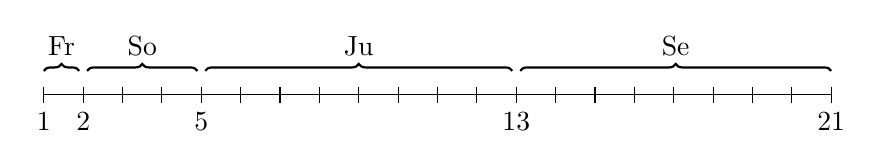
\begin{tikzpicture}
    \draw (1/2,0) -- (21/2,0);
    \foreach \i in {1,2,5,13,21} {\draw (\i/2,0.1) -- + (0,-0.2) node[below] {$\i$};}
    \foreach \i in {1,2,...,21} {\draw (\i/2,0.1) -- + (0,-0.2);}
    \draw[decorate, decoration={brace}, yshift=2ex, thick]  (1/2,0) -- node[above=0.4ex] {$\mathrm{Fr}$}  (1.9/2,0);
    \draw[decorate, decoration={brace}, yshift=2ex, thick]  (2.1/2,0) -- node[above=0.4ex] {$\mathrm{So}$}  (4.9/2,0);
    \draw[decorate, decoration={brace}, yshift=2ex, thick]  (5.1/2,0) -- node[above=0.4ex] {$\mathrm{Ju}$}  (12.9/2,0);
    \draw[decorate, decoration={brace}, yshift=2ex, thick]  (13.1/2,0) -- node[above=0.4ex] {$\mathrm{Se}$}  (21/2,0);
    \end{tikzpicture}
    \end{center}
$\Box$
\end{example}

While the exponential mechanism is a general-purpose technique for sampling from a distribution defined by a utility function, it is not the only one. In fact, it is possible to show that the exponential mechanism is optimal in the sense that it minimizes the probability of error in the output. However, it is not always the most efficient. For example, if the utility function is linear, then we can use a simpler technique called \textbf{Laplace noise} to sample from the distribution. We'll discuss this technique in the next section.

\subsection{Adding Noise} 
The first approach we'll discuss is based on adding ``noise'', or carefully-chosen random values, to the result of a computation. In particular, we'll begin by computing the exact result, and then add noise before releasing it. 
Global sensitivity bounds the magnitude by which \san's response can change on pairs of neighboring databases. Our goal in designing a differentially-private version of \san is to hide such changes, so that the function's response on neighboring pairs is approximately the same. Thus, $\Delta\san$ tells us how much noise we need to add to the result to do so.

\paragraph{Laplace noise.}
The key to finding the right noise to add is in selecting an appropriate distribution to sample from. We'll use the \textbf{Laplace distribution} with parameter $b$, denoted $\lap(b)$, which has density function:
\begin{equation}
\label{eq:lap}
\mathbf{Pr}[z] = \frac{1}{2b}\exp\left(\frac{-|z|}{b}\right)
\end{equation}
Alternatively, the density function for $\lap(b)$ can be given as:
\begin{equation}
\label{eq:lap2}
\mathbf{Pr}[z] = 
\frac{1}{2b}
\left\{
\begin{array}{ll}
%
\exp\left(\frac{z}{b}\right) & \mathrm{if\ } x < 0 \\
\exp\left(\frac{-z}{b}\right) & \mathrm{if\ } x \ge 0 
\end{array}
\right.
\end{equation}

\begin{figure}
\centering
\begin{tikzpicture}
\begin{axis}[every axis plot post/.append style={
  mark=none,domain=-10:10,samples=400,smooth}, % All plots: from -2:2, 50 samples, smooth, no marks
  axis x line*=bottom, % no box around the plot, only x and y axis
  axis y line*=left, % the * suppresses the arrow tips
  enlargelimits=upper] % extend the axes a bit to the right and top
  \addplot {laplace(0.5)};
  \addplot {laplace(2)};
\end{axis}
\end{tikzpicture}
\label{fig:laplace}
\caption{Laplace distribution with $b=\frac{1}{2}$ (blue) and $b = 2$ (red).}
\end{figure}

The Laplace distribution is shown in Figure~\ref{fig:laplace}. There are several important points to note about its shape.
\begin{itemize}
\item The distribution is centered (i.e., has its mean) at 0 and is symmetric. Because we're going to add samples from this distribution to our response, both of these properties are important. If the distribution were biased (i.e., its mean were something other than 0), then on average we would unnecessarily skew the results of \san by offsetting them by the distribution's mean. The symmetric property of $\lap(b)$ means that the noisy result is no more likey to be greater (or smaller) than the true result. If the distribution only had support in the positive half-space of $\mathbb{R}$, for example, then the only databases for which $\mathsf{count}(X,e)$ could return 0 would be those with no rows satisfying $e$. A user who is aware of this fact could leverage it to learn more about $X$ than we want to provide in our response.

\item Most of the mass in this distribution is close to 0. In fact, looking at Equation~\ref{eq:lap}, the probability of sampling a value $z$ drops off exponentially as $z$ moves further from 0, so drawing a very large or small value is exceedingly unlikely. This is good for accuracy, because it means that the noise we add will have small magnitude most of the time.

\item Notice in Figure~\ref{fig:laplace} that the shape of the distribution for $b=2$ is quite a bit ``flatter'' than the one for $b=0.5$. If we were to add noise from $\lap(2)$, then our response will on average diverge more from the true answer than they would for $\lap(0.5)$. While $\lap(2)$ is clearly worse in terms of utility, it offers stronger privacy. We will exploit this fact by relating the parameter $b$ to the privacy budget $\epsilon$ when we generate noise.
\end{itemize}

Now that we have some intuition for the Laplace distribution, we can show how it is used to make \san differentially-private.

\begin{theorem}{(Dwork et al., 2006)}
\label{thm:noise}
Assume that \san is a function $\san : \mathbf{X} \mapsto \mathbb{R}$. Then the function
\[
\psan(X) = \san(X) + \lap\left(\frac{\Delta\san}{\epsilon}\right)
\]
satisfies $\epsilon$-differential privacy.
\end{theorem}

Theorem~\ref{thm:noise} describes the \textbf{Laplace mechanism}, a general strategy for obtaining differentially-private functions by the addition of noise.

\section{Composing Differentially-Private Computations}

There are many algorithms beyond randomized response that have been rigorously shown to satisfy differential privacy. Indeed, we could fill at least one semester-long course covering only a subset of them, and our goals in this class are more broad. If you are interested in this topic, then please consult the papers in the references section of these notes~\cite{Chaudhuri2011,ErlingssonKP14,McSherry2009}, and in particular the text by Cynthia Dwork and Aaron Roth~\cite{Dwork2014}, for more on these algorithms.

For the rest of the lecture, we will assume that we are in possession of a algorithm $\asprg_1, \ldots, \asprg_n$ that have already been shown to be differentially private. Our goal is to use them through some composition to implement a larger program that we can by extension show satisfies differential privacy. To support this, we will develop a set of \emph{composition theorems} that allow us to draw such conclusions from the assumption that sub-components satisfy $\epsilon_i$-DP.

\paragraph{Post-processing.} The first important property we'll discuss covers post-processing, or computations that are performed that take the result of a differentially-private function as input. Differential privacy enjoys a post-processing guarantee when the post-processor is deterministic, as shown in Theorem~\ref{thm:post}.

\begin{theorem}{Post-processing.}
\label{thm:post}
Let $\san : \mathbf{X} \mapsto \mathbf{Y}$ be a randomized $\epsilon$-differentially private function, and $f : \mathbf{Y} \mapsto \mathbf{Y}$ be any deterministic function. Then $f \circ \san$ is $\epsilon$-differentially private.
\end{theorem}

\begin{proof}
Let $X_1, X_2$ be neighboring inputs, and $Y \in \mathbf{Y}$ be any output of $f$. Let $I \in \mathbf{Y}$ be such that $f(I) = Y$. Then,
\begin{align*}
\mathrm{Pr}[f(\san(X_1)) = Y] &= \mathrm{Pr}[\san(X_1) = I] \\
&\le e^\epsilon\mathrm{Pr}[\san(X_2) = I] \\
&= e^\epsilon\mathrm{Pr}[f(\san(X_2)) = Y]
\end{align*}
\end{proof}

The usefulness of the post-processing theorem is apparent: we can always perform deterministic computations over data produced by $\epsilon$-DP computations, and still arrive at $\epsilon$-DP results. Intuitively, the information content of a signal cannot be increased by local deterministic processing. If the input to $f$ contains no information about an individual, then $f$ cannot add any.

\paragraph{Sequential composition.} The next type of composition that we'll consider applies a sequence of functions $\san_i$, each of which provide $\epsilon_i$-differential privacy, and releases the union of their results. We can still obtain a privacy guarantee, but the budgets increase additively.

\begin{theorem}{(Sequential Composition~\cite{McSherry2009})}
Let $\san_i : \mathbf{X} \mapsto \mathbf{Y}$, $1 \le i \le n$ be a sequence of $n$ randomized $\epsilon_i$-differentially private functions, and let $\san(X) = (\san_1(X), \ldots, \san_n(X))$. Then \san is $(\sum_{1 \le i \le n} \epsilon_i)$-differentially private.
\end{theorem}

\begin{proof}
Let $O \in \mathbf{Y}^n$ be some value in the range of \san, and $X_1, X_2$ be neighboring inputs. Then we can simply calculate:
\begin{align*}
\frac{
  \mathrm{Pr}[\san(X_1) = O]
}{
  \mathrm{Pr}[\san(X_2) = O]
}
&=
\frac{
  \prod_{1 \le i \le n} \mathrm{Pr}[\san_i(X_1) = O]
}{
  \prod_{1 \le i \le n} \mathrm{Pr}[\san_i(X_2) = O]
}
\\
&=
\left(
\frac{
  \mathrm{Pr}[\san_1(X_1) = O]
}{
  \mathrm{Pr}[\san_1(X_2) = O]
}
\right)
\cdots
\left(
\frac{
  \mathrm{Pr}[\san_n(X_1) = O]
}{
  \mathrm{Pr}[\san_n(X_2) = O]
}
\right)
\\
&\le
e^{\epsilon_1}\cdots e^{\epsilon_n}
\\
&=
e^{\epsilon_1 + \cdots + \epsilon_n}
\end{align*}
\end{proof}

The sequential composition theorem is crucial for any practical system that hopes to achieve differential privacy. Notably, it implies that for a fixed privacy budget $\epsilon$, it isn't safe to apply a differentially-private computation an arbitrary number of times to the same input $X$. If the total sum of the computations' budgets exceeds $\epsilon$, then the composed computation is no longer $\epsilon$-differentially private. If we want to ensure a certain level of privacy in a computation composed of multiple queries, then we need to carefully account for the amount of privacy budget that is ``consumed''  by each query. If the amount ever exceeds our budget, then we can never answer another query from that input.

\paragraph{Parallel composition.} The last form of composition that we'll look at is targeted towards the use of multiple differentially-private queries over \textbf{disjoint} partitions of $X$.

\begin{theorem}{(Parallel Composition~\cite{McSherry2009})}
Let $\san_i : \mathbf{X} \mapsto \mathbf{Y}$, $1 \le i \le n$ be a sequence of $n$ randomized $\epsilon_i$-differentially private functions, $P_1, \ldots, P_n$ be disjoint subsets of $X$, and let $\san(X) = (\san_1(P_1), \ldots, \san_n(P_n))$. Then \san is $(\max_{1 \le i \le n} \epsilon_i)$-differentially private.
\end{theorem}

\begin{proof}
Let $O \in \mathbf{Y}^n$ be some value in the range of \san, and $X_1, X_2$ be neighboring inputs. Let $P_{1,1}, \ldots, P_{1,n}$ be the disjoint subsets of $X_1$, and $P_{2,1}, \ldots, P_{2,n}$ similarly for $X_2$. Observe that there is only one partition index, $i$, at which $P_{1,i}$ and $P_{2,i}$ differ. Assume without loss of generality that the index is $1$. Then:
\begin{align*}
\frac{
  \mathrm{Pr}[\san(X_1) = O]
}{
  \mathrm{Pr}[\san(X_2) = O]
}
&=
\frac{
  \prod_{1 \le i \le n} \mathrm{Pr}[\san_i(P_{1,i}) = O]
}{
  \prod_{1 \le i \le n} \mathrm{Pr}[\san_i(P_{2,i}) = O]
}
\\
&=
\frac{
  \mathrm{Pr}[\san_1(X_1) = O]
}{
  \mathrm{Pr}[\san_1(X_2) = O]
}
\\
&\le
\max_{1 \le i \le n} \epsilon_i
\end{align*}
The second line follows because we assumed that the differing index occured in the first partition, so:
\[
\prod_{2 \le i \le n} \mathrm{Pr}[\san_i(P_{1,i}) = O] = \prod_{2 \le i \le n} \mathrm{Pr}[\san_i(P_{2,i}) = O]
\]
The last line follows under the pessimistic assumption that the largest $\epsilon_i$ applies to the first partition.
\end{proof}

Parallel composition is probably not as widely applicable as the sequential form, but can be very useful in certain cases because it does not expend privacy budget additively. Whenever computations can be broken into smaller sub-computations over disjoint data, applying the parallel composition theorem followed by post-processing can lead to strong utility for a fixed privacy budget.

\bibliographystyle{abbrv}
\bibliography{bibliography}
\end{document}